% Options for packages loaded elsewhere
\PassOptionsToPackage{unicode}{hyperref}
\PassOptionsToPackage{hyphens}{url}
\PassOptionsToPackage{dvipsnames,svgnames,x11names}{xcolor}
%
\documentclass[
  a4paperpaper,
]{article}

\usepackage{amsmath,amssymb}
\usepackage{iftex}
\ifPDFTeX
  \usepackage[T1]{fontenc}
  \usepackage[utf8]{inputenc}
  \usepackage{textcomp} % provide euro and other symbols
\else % if luatex or xetex
  \ifXeTeX
    \usepackage{mathspec} % this also loads fontspec
  \else
    \usepackage{unicode-math} % this also loads fontspec
  \fi
  \defaultfontfeatures{Scale=MatchLowercase}
  \defaultfontfeatures[\rmfamily]{Ligatures=TeX,Scale=1}
\fi
\usepackage{lmodern}
\ifPDFTeX\else  
    % xetex/luatex font selection
\fi
% Use upquote if available, for straight quotes in verbatim environments
\IfFileExists{upquote.sty}{\usepackage{upquote}}{}
\IfFileExists{microtype.sty}{% use microtype if available
  \usepackage[]{microtype}
  \UseMicrotypeSet[protrusion]{basicmath} % disable protrusion for tt fonts
}{}
\makeatletter
\@ifundefined{KOMAClassName}{% if non-KOMA class
  \IfFileExists{parskip.sty}{%
    \usepackage{parskip}
  }{% else
    \setlength{\parindent}{0pt}
    \setlength{\parskip}{6pt plus 2pt minus 1pt}}
}{% if KOMA class
  \KOMAoptions{parskip=half}}
\makeatother
\usepackage{xcolor}
\usepackage[top=30mm,left=30mm,right=30mm,heightrounded]{geometry}
\setlength{\emergencystretch}{3em} % prevent overfull lines
\setcounter{secnumdepth}{5}
% Make \paragraph and \subparagraph free-standing
\ifx\paragraph\undefined\else
  \let\oldparagraph\paragraph
  \renewcommand{\paragraph}[1]{\oldparagraph{#1}\mbox{}}
\fi
\ifx\subparagraph\undefined\else
  \let\oldsubparagraph\subparagraph
  \renewcommand{\subparagraph}[1]{\oldsubparagraph{#1}\mbox{}}
\fi

\usepackage{color}
\usepackage{fancyvrb}
\newcommand{\VerbBar}{|}
\newcommand{\VERB}{\Verb[commandchars=\\\{\}]}
\DefineVerbatimEnvironment{Highlighting}{Verbatim}{commandchars=\\\{\}}
% Add ',fontsize=\small' for more characters per line
\usepackage{framed}
\definecolor{shadecolor}{RGB}{241,243,245}
\newenvironment{Shaded}{\begin{snugshade}}{\end{snugshade}}
\newcommand{\AlertTok}[1]{\textcolor[rgb]{0.68,0.00,0.00}{#1}}
\newcommand{\AnnotationTok}[1]{\textcolor[rgb]{0.37,0.37,0.37}{#1}}
\newcommand{\AttributeTok}[1]{\textcolor[rgb]{0.40,0.45,0.13}{#1}}
\newcommand{\BaseNTok}[1]{\textcolor[rgb]{0.68,0.00,0.00}{#1}}
\newcommand{\BuiltInTok}[1]{\textcolor[rgb]{0.00,0.23,0.31}{#1}}
\newcommand{\CharTok}[1]{\textcolor[rgb]{0.13,0.47,0.30}{#1}}
\newcommand{\CommentTok}[1]{\textcolor[rgb]{0.37,0.37,0.37}{#1}}
\newcommand{\CommentVarTok}[1]{\textcolor[rgb]{0.37,0.37,0.37}{\textit{#1}}}
\newcommand{\ConstantTok}[1]{\textcolor[rgb]{0.56,0.35,0.01}{#1}}
\newcommand{\ControlFlowTok}[1]{\textcolor[rgb]{0.00,0.23,0.31}{#1}}
\newcommand{\DataTypeTok}[1]{\textcolor[rgb]{0.68,0.00,0.00}{#1}}
\newcommand{\DecValTok}[1]{\textcolor[rgb]{0.68,0.00,0.00}{#1}}
\newcommand{\DocumentationTok}[1]{\textcolor[rgb]{0.37,0.37,0.37}{\textit{#1}}}
\newcommand{\ErrorTok}[1]{\textcolor[rgb]{0.68,0.00,0.00}{#1}}
\newcommand{\ExtensionTok}[1]{\textcolor[rgb]{0.00,0.23,0.31}{#1}}
\newcommand{\FloatTok}[1]{\textcolor[rgb]{0.68,0.00,0.00}{#1}}
\newcommand{\FunctionTok}[1]{\textcolor[rgb]{0.28,0.35,0.67}{#1}}
\newcommand{\ImportTok}[1]{\textcolor[rgb]{0.00,0.46,0.62}{#1}}
\newcommand{\InformationTok}[1]{\textcolor[rgb]{0.37,0.37,0.37}{#1}}
\newcommand{\KeywordTok}[1]{\textcolor[rgb]{0.00,0.23,0.31}{#1}}
\newcommand{\NormalTok}[1]{\textcolor[rgb]{0.00,0.23,0.31}{#1}}
\newcommand{\OperatorTok}[1]{\textcolor[rgb]{0.37,0.37,0.37}{#1}}
\newcommand{\OtherTok}[1]{\textcolor[rgb]{0.00,0.23,0.31}{#1}}
\newcommand{\PreprocessorTok}[1]{\textcolor[rgb]{0.68,0.00,0.00}{#1}}
\newcommand{\RegionMarkerTok}[1]{\textcolor[rgb]{0.00,0.23,0.31}{#1}}
\newcommand{\SpecialCharTok}[1]{\textcolor[rgb]{0.37,0.37,0.37}{#1}}
\newcommand{\SpecialStringTok}[1]{\textcolor[rgb]{0.13,0.47,0.30}{#1}}
\newcommand{\StringTok}[1]{\textcolor[rgb]{0.13,0.47,0.30}{#1}}
\newcommand{\VariableTok}[1]{\textcolor[rgb]{0.07,0.07,0.07}{#1}}
\newcommand{\VerbatimStringTok}[1]{\textcolor[rgb]{0.13,0.47,0.30}{#1}}
\newcommand{\WarningTok}[1]{\textcolor[rgb]{0.37,0.37,0.37}{\textit{#1}}}

\providecommand{\tightlist}{%
  \setlength{\itemsep}{0pt}\setlength{\parskip}{0pt}}\usepackage{longtable,booktabs,array}
\usepackage{calc} % for calculating minipage widths
% Correct order of tables after \paragraph or \subparagraph
\usepackage{etoolbox}
\makeatletter
\patchcmd\longtable{\par}{\if@noskipsec\mbox{}\fi\par}{}{}
\makeatother
% Allow footnotes in longtable head/foot
\IfFileExists{footnotehyper.sty}{\usepackage{footnotehyper}}{\usepackage{footnote}}
\makesavenoteenv{longtable}
\usepackage{graphicx}
\makeatletter
\def\maxwidth{\ifdim\Gin@nat@width>\linewidth\linewidth\else\Gin@nat@width\fi}
\def\maxheight{\ifdim\Gin@nat@height>\textheight\textheight\else\Gin@nat@height\fi}
\makeatother
% Scale images if necessary, so that they will not overflow the page
% margins by default, and it is still possible to overwrite the defaults
% using explicit options in \includegraphics[width, height, ...]{}
\setkeys{Gin}{width=\maxwidth,height=\maxheight,keepaspectratio}
% Set default figure placement to htbp
\makeatletter
\def\fps@figure{htbp}
\makeatother

\usepackage{fvextra}
\DefineVerbatimEnvironment{Highlighting}{Verbatim}{breaklines,commandchars=\\\{\}}
\DefineVerbatimEnvironment{OutputCode}{Verbatim}{breaklines,commandchars=\\\{\}}
\makeatletter
\@ifpackageloaded{caption}{}{\usepackage{caption}}
\AtBeginDocument{%
\ifdefined\contentsname
  \renewcommand*\contentsname{Índice}
\else
  \newcommand\contentsname{Índice}
\fi
\ifdefined\listfigurename
  \renewcommand*\listfigurename{Lista de Figuras}
\else
  \newcommand\listfigurename{Lista de Figuras}
\fi
\ifdefined\listtablename
  \renewcommand*\listtablename{Lista de Tabelas}
\else
  \newcommand\listtablename{Lista de Tabelas}
\fi
\ifdefined\figurename
  \renewcommand*\figurename{Figura}
\else
  \newcommand\figurename{Figura}
\fi
\ifdefined\tablename
  \renewcommand*\tablename{Tabela}
\else
  \newcommand\tablename{Tabela}
\fi
}
\@ifpackageloaded{float}{}{\usepackage{float}}
\floatstyle{ruled}
\@ifundefined{c@chapter}{\newfloat{codelisting}{h}{lop}}{\newfloat{codelisting}{h}{lop}[chapter]}
\floatname{codelisting}{Listagem}
\newcommand*\listoflistings{\listof{codelisting}{Lista de Listagens}}
\makeatother
\makeatletter
\makeatother
\makeatletter
\@ifpackageloaded{caption}{}{\usepackage{caption}}
\@ifpackageloaded{subcaption}{}{\usepackage{subcaption}}
\makeatother
\ifLuaTeX
\usepackage[bidi=basic]{babel}
\else
\usepackage[bidi=default]{babel}
\fi
\babelprovide[main,import]{portuguese}
% get rid of language-specific shorthands (see #6817):
\let\LanguageShortHands\languageshorthands
\def\languageshorthands#1{}
\ifLuaTeX
  \usepackage{selnolig}  % disable illegal ligatures
\fi
\usepackage{bookmark}

\IfFileExists{xurl.sty}{\usepackage{xurl}}{} % add URL line breaks if available
\urlstyle{same} % disable monospaced font for URLs
\hypersetup{
  pdftitle={Lista 2: Dropout e Keras},
  pdfauthor={César A. Galvão - 190011572},
  pdflang={pt},
  colorlinks=true,
  linkcolor={blue},
  filecolor={Maroon},
  citecolor={Blue},
  urlcolor={Blue},
  pdfcreator={LaTeX via pandoc}}

\title{Lista 2: Dropout e Keras}
\author{César A. Galvão - 190011572}
\date{}

\begin{document}
\maketitle

\section{Questão 1}\label{questuxe3o-1}

\subsection{Item a)}\label{sec-1a}

Altere seu código da Lista 1 (ou, se preferir, os códigos
disponibilizados como gabarito) para implementar a técnica dropout na
camada de entrada e na camada intermediária. Use \(p = 0,6\), onde \(p\)
representa a probabilidade de inclusão de cada neurônio. Atenção: neste
item, não é preciso calcular o custo da rede no conjunto de validação!

A cada nova iteração do algoritmo de otimização, a rede neural corrente
gera estimativas pontuais aleatórias para as observações do conjunto de
treinamento. Essas estimativas, por sua vez, são usadas para calcular o
custo no conjunto de treinamento e atualizar os pesos da rede.

Reporte o menor custo observado durante o treinamento e salve os
respectivos pesos para responder os demais itens da Questão 1.

\begin{center}\rule{0.5\linewidth}{0.5pt}\end{center}

~

A seguir é utilizado o código do gabarito da Lista 1, acrescido de uma
alteração na função de \emph{backpropagation} para incluir o dropout às
unidades \(x_1, x_2, h_1\) e \(h_2\). O dropout é implementado por meio
de uma máscara binária que é aplicada a cada unidade com probabilidade
\(p = 0,6\), gerada a cada iteração com o uso de \texttt{rbinom()}. A
máscara é aplicada matricialmente a \(\mathbf{X}\) e \(\mathbf{h}\).

~

\begin{Shaded}
\begin{Highlighting}[]
\CommentTok{\# funcoes de apoio {-}{-}{-}{-}}
\NormalTok{sigmoide }\OtherTok{\textless{}{-}} \ControlFlowTok{function}\NormalTok{(x) \{}
  \FunctionTok{return}\NormalTok{(}\DecValTok{1}\SpecialCharTok{/}\NormalTok{(}\DecValTok{1}\SpecialCharTok{+}\FunctionTok{exp}\NormalTok{(}\SpecialCharTok{{-}}\NormalTok{x)))}
\NormalTok{\}}

\NormalTok{derivada\_sigmoide }\OtherTok{\textless{}{-}} \ControlFlowTok{function}\NormalTok{(x) \{}
  \FunctionTok{return}\NormalTok{(}\FunctionTok{exp}\NormalTok{(}\SpecialCharTok{{-}}\NormalTok{x)}\SpecialCharTok{/}\NormalTok{((}\DecValTok{1}\SpecialCharTok{+}\FunctionTok{exp}\NormalTok{(}\SpecialCharTok{{-}}\NormalTok{x))}\SpecialCharTok{\^{}}\DecValTok{2}\NormalTok{))}
\NormalTok{\}}

\NormalTok{mse\_cost }\OtherTok{\textless{}{-}} \ControlFlowTok{function}\NormalTok{(y\_true, y\_hat) \{}
  \FunctionTok{return}\NormalTok{(}\FunctionTok{mean}\NormalTok{((y\_true }\SpecialCharTok{{-}}\NormalTok{ y\_hat)}\SpecialCharTok{\^{}}\DecValTok{2}\NormalTok{))}
\NormalTok{\}}

\CommentTok{\# forward propagation {-}{-}{-}{-}}
\NormalTok{feed\_forward }\OtherTok{\textless{}{-}} \ControlFlowTok{function}\NormalTok{(theta, x) \{}
\CommentTok{\# Transformação de x para um formato de matriz}
  \FunctionTok{ifelse}\NormalTok{(}\FunctionTok{is.double}\NormalTok{(x), x }\OtherTok{\textless{}{-}} \FunctionTok{as.matrix}\NormalTok{(x), x }\OtherTok{\textless{}{-}} \FunctionTok{t}\NormalTok{(}\FunctionTok{as.matrix}\NormalTok{(x)))}
  
  \CommentTok{\# Extração dos parâmetros}
\NormalTok{  W1 }\OtherTok{\textless{}{-}} \FunctionTok{matrix}\NormalTok{(}\AttributeTok{data =}\NormalTok{ theta[}\DecValTok{1}\SpecialCharTok{:}\DecValTok{4}\NormalTok{], }\AttributeTok{nrow =} \DecValTok{2}\NormalTok{)}
\NormalTok{  W2 }\OtherTok{\textless{}{-}} \FunctionTok{matrix}\NormalTok{(}\AttributeTok{data =}\NormalTok{ theta[}\DecValTok{5}\SpecialCharTok{:}\DecValTok{6}\NormalTok{], }\AttributeTok{nrow =} \DecValTok{2}\NormalTok{)}
\NormalTok{  b1 }\OtherTok{\textless{}{-}}\NormalTok{ theta[}\DecValTok{7}\SpecialCharTok{:}\DecValTok{8}\NormalTok{]}
\NormalTok{  b2 }\OtherTok{\textless{}{-}}\NormalTok{ theta[}\DecValTok{9}\NormalTok{]}
  \CommentTok{\# Camada escondida}
\NormalTok{  a }\OtherTok{\textless{}{-}} \FunctionTok{matrix}\NormalTok{(}\AttributeTok{data =} \FunctionTok{rep}\NormalTok{(b1, }\FunctionTok{ncol}\NormalTok{(x)), }\AttributeTok{nrow =} \DecValTok{2}\NormalTok{) }\SpecialCharTok{+}\NormalTok{ W1 }\SpecialCharTok{\%*\%}\NormalTok{ x}
\NormalTok{  h }\OtherTok{\textless{}{-}} \FunctionTok{sigmoide}\NormalTok{(a)}
  
  
  \CommentTok{\# Previsão}
\NormalTok{  y\_hat }\OtherTok{\textless{}{-}} \FunctionTok{as.double}\NormalTok{(b2 }\SpecialCharTok{+} \FunctionTok{t}\NormalTok{(W2) }\SpecialCharTok{\%*\%}\NormalTok{ h)}
  \FunctionTok{return}\NormalTok{(y\_hat)}
\NormalTok{\}}

\NormalTok{feed\_forward\_drop }\OtherTok{\textless{}{-}} \ControlFlowTok{function}\NormalTok{(theta, x, }\AttributeTok{drop\_rate =} \FloatTok{0.6}\NormalTok{) \{}
\CommentTok{\# Transformação de x para um formato de matriz}
  \FunctionTok{ifelse}\NormalTok{(}\FunctionTok{is.double}\NormalTok{(x), x }\OtherTok{\textless{}{-}} \FunctionTok{as.matrix}\NormalTok{(x), x }\OtherTok{\textless{}{-}} \FunctionTok{t}\NormalTok{(}\FunctionTok{as.matrix}\NormalTok{(x)))}
  
  \CommentTok{\#gera mascaras}
\NormalTok{  mask }\OtherTok{\textless{}{-}} \FunctionTok{replicate}\NormalTok{(}\FunctionTok{dim}\NormalTok{(x)[}\DecValTok{2}\NormalTok{],}\FunctionTok{rbinom}\NormalTok{(}\DecValTok{4}\NormalTok{, }\DecValTok{1}\NormalTok{, drop\_rate))}
  \CommentTok{\#aplica mascaras}
\NormalTok{  x }\OtherTok{\textless{}{-}}\NormalTok{ x }\SpecialCharTok{*}\NormalTok{ mask[}\DecValTok{1}\SpecialCharTok{:}\DecValTok{2}\NormalTok{,]}
  
  \CommentTok{\# Extração dos parâmetros}
\NormalTok{  W1 }\OtherTok{\textless{}{-}} \FunctionTok{matrix}\NormalTok{(}\AttributeTok{data =}\NormalTok{ theta[}\DecValTok{1}\SpecialCharTok{:}\DecValTok{4}\NormalTok{], }\AttributeTok{nrow =} \DecValTok{2}\NormalTok{)}
\NormalTok{  W2 }\OtherTok{\textless{}{-}} \FunctionTok{matrix}\NormalTok{(}\AttributeTok{data =}\NormalTok{ theta[}\DecValTok{5}\SpecialCharTok{:}\DecValTok{6}\NormalTok{], }\AttributeTok{nrow =} \DecValTok{2}\NormalTok{)}
\NormalTok{  b1 }\OtherTok{\textless{}{-}}\NormalTok{ theta[}\DecValTok{7}\SpecialCharTok{:}\DecValTok{8}\NormalTok{]}
\NormalTok{  b2 }\OtherTok{\textless{}{-}}\NormalTok{ theta[}\DecValTok{9}\NormalTok{]}
  \CommentTok{\# Camada escondida}
\NormalTok{  a }\OtherTok{\textless{}{-}} \FunctionTok{matrix}\NormalTok{(}\AttributeTok{data =} \FunctionTok{rep}\NormalTok{(b1, }\FunctionTok{ncol}\NormalTok{(x)), }\AttributeTok{nrow =} \DecValTok{2}\NormalTok{) }\SpecialCharTok{+}\NormalTok{ W1 }\SpecialCharTok{\%*\%}\NormalTok{ x}
\NormalTok{  h }\OtherTok{\textless{}{-}} \FunctionTok{sigmoide}\NormalTok{(a)}
  
  \CommentTok{\#aplica mascaras}
\NormalTok{  h }\OtherTok{\textless{}{-}}\NormalTok{ h }\SpecialCharTok{*}\NormalTok{ mask[}\DecValTok{3}\SpecialCharTok{:}\DecValTok{4}\NormalTok{,]  }
  
  \CommentTok{\# Previsão}
\NormalTok{  y\_hat }\OtherTok{\textless{}{-}} \FunctionTok{as.double}\NormalTok{(b2 }\SpecialCharTok{+} \FunctionTok{t}\NormalTok{(W2) }\SpecialCharTok{\%*\%}\NormalTok{ h)}
  \FunctionTok{return}\NormalTok{(y\_hat)}
\NormalTok{\}}


\NormalTok{feed\_forward\_scale }\OtherTok{\textless{}{-}} \ControlFlowTok{function}\NormalTok{(theta, x, }\AttributeTok{scale =} \FloatTok{0.6}\NormalTok{) \{}
\CommentTok{\# Transformação de x para um formato de matriz}
  \FunctionTok{ifelse}\NormalTok{(}\FunctionTok{is.double}\NormalTok{(x), x }\OtherTok{\textless{}{-}} \FunctionTok{as.matrix}\NormalTok{(x), x }\OtherTok{\textless{}{-}} \FunctionTok{t}\NormalTok{(}\FunctionTok{as.matrix}\NormalTok{(x)))}
  
  \CommentTok{\# \#gera mascaras}
  \CommentTok{\# mask \textless{}{-} replicate(dim(x)[2],rbinom(4, 1, drop\_rate))}
  \CommentTok{\# \#aplica mascaras}
  \CommentTok{\# x \textless{}{-} x * mask[1:2,]}
  
  \CommentTok{\# Extração dos parâmetros}
\NormalTok{  W1 }\OtherTok{\textless{}{-}} \FunctionTok{matrix}\NormalTok{(}\AttributeTok{data =}\NormalTok{ theta[}\DecValTok{1}\SpecialCharTok{:}\DecValTok{4}\NormalTok{], }\AttributeTok{nrow =} \DecValTok{2}\NormalTok{)}
\NormalTok{  W2 }\OtherTok{\textless{}{-}} \FunctionTok{matrix}\NormalTok{(}\AttributeTok{data =}\NormalTok{ theta[}\DecValTok{5}\SpecialCharTok{:}\DecValTok{6}\NormalTok{], }\AttributeTok{nrow =} \DecValTok{2}\NormalTok{)}
\NormalTok{  scaled\_W1 }\OtherTok{\textless{}{-}}\NormalTok{ (scale) }\SpecialCharTok{*}\NormalTok{ W1}
\NormalTok{  scaled\_W2 }\OtherTok{\textless{}{-}}\NormalTok{ (scale) }\SpecialCharTok{*}\NormalTok{ W2}
\NormalTok{  b1 }\OtherTok{\textless{}{-}}\NormalTok{ theta[}\DecValTok{7}\SpecialCharTok{:}\DecValTok{8}\NormalTok{]}
\NormalTok{  b2 }\OtherTok{\textless{}{-}}\NormalTok{ theta[}\DecValTok{9}\NormalTok{]}
  \CommentTok{\# Camada escondida}
\NormalTok{  a }\OtherTok{\textless{}{-}} \FunctionTok{matrix}\NormalTok{(}\AttributeTok{data =} \FunctionTok{rep}\NormalTok{(b1, }\FunctionTok{ncol}\NormalTok{(x)), }\AttributeTok{nrow =} \DecValTok{2}\NormalTok{) }\SpecialCharTok{+}\NormalTok{ W1 }\SpecialCharTok{\%*\%}\NormalTok{ x}
\NormalTok{  h }\OtherTok{\textless{}{-}} \FunctionTok{sigmoide}\NormalTok{(a)}
  
  \CommentTok{\# \#aplica mascaras}
  \CommentTok{\# h \textless{}{-} h * mask[3:4,]  }
  
  \CommentTok{\# Previsão}
\NormalTok{  y\_hat }\OtherTok{\textless{}{-}} \FunctionTok{as.double}\NormalTok{(b2 }\SpecialCharTok{+} \FunctionTok{t}\NormalTok{(W2) }\SpecialCharTok{\%*\%}\NormalTok{ h)}
  \FunctionTok{return}\NormalTok{(y\_hat)}
\NormalTok{\}}



\CommentTok{\# back propagation {-}{-}{-}{-}}
\CommentTok{\# para as epochs, é necessário rodar um for}
\NormalTok{back\_prop\_drop }\OtherTok{\textless{}{-}} \ControlFlowTok{function}\NormalTok{(theta, x, y, }\AttributeTok{drop\_rate =} \FloatTok{0.6}\NormalTok{)\{}

  \DocumentationTok{\#\#\# Primeiro, deve{-}se realizar o forward propagation}
  \FunctionTok{ifelse}\NormalTok{(}\FunctionTok{is.double}\NormalTok{(x), x }\OtherTok{\textless{}{-}} \FunctionTok{as.matrix}\NormalTok{(x), x }\OtherTok{\textless{}{-}} \FunctionTok{t}\NormalTok{(}\FunctionTok{as.matrix}\NormalTok{(x)))}
  
    \CommentTok{\#gera mascaras}
\NormalTok{    mask }\OtherTok{\textless{}{-}} \FunctionTok{replicate}\NormalTok{(}\FunctionTok{dim}\NormalTok{(x)[}\DecValTok{2}\NormalTok{],}\FunctionTok{rbinom}\NormalTok{(}\DecValTok{4}\NormalTok{, }\DecValTok{1}\NormalTok{, drop\_rate))}
    \CommentTok{\#aplica mascaras}
\NormalTok{    x }\OtherTok{\textless{}{-}}\NormalTok{ x }\SpecialCharTok{*}\NormalTok{ mask[}\DecValTok{1}\SpecialCharTok{:}\DecValTok{2}\NormalTok{,]}
  
\NormalTok{  W1 }\OtherTok{\textless{}{-}} \FunctionTok{matrix}\NormalTok{(}\AttributeTok{data =}\NormalTok{ theta[}\DecValTok{1}\SpecialCharTok{:}\DecValTok{4}\NormalTok{], }\AttributeTok{nrow =} \DecValTok{2}\NormalTok{)}
\NormalTok{  W2 }\OtherTok{\textless{}{-}} \FunctionTok{matrix}\NormalTok{(}\AttributeTok{data =}\NormalTok{ theta[}\DecValTok{5}\SpecialCharTok{:}\DecValTok{6}\NormalTok{], }\AttributeTok{nrow =} \DecValTok{2}\NormalTok{)}
\NormalTok{  b1 }\OtherTok{\textless{}{-}}\NormalTok{ theta[}\DecValTok{7}\SpecialCharTok{:}\DecValTok{8}\NormalTok{]}
\NormalTok{  b2 }\OtherTok{\textless{}{-}}\NormalTok{ theta[}\DecValTok{9}\NormalTok{]}
\NormalTok{  a }\OtherTok{\textless{}{-}} \FunctionTok{matrix}\NormalTok{(}\AttributeTok{data =} \FunctionTok{rep}\NormalTok{(b1, }\FunctionTok{ncol}\NormalTok{(x)), }\AttributeTok{nrow =} \DecValTok{2}\NormalTok{) }\SpecialCharTok{+}\NormalTok{ W1 }\SpecialCharTok{\%*\%}\NormalTok{ x}
\NormalTok{  h }\OtherTok{\textless{}{-}} \FunctionTok{sigmoide}\NormalTok{(a)}
    
  \CommentTok{\#aplica mascaras}
\NormalTok{  h }\OtherTok{\textless{}{-}}\NormalTok{ h }\SpecialCharTok{*}\NormalTok{ mask[}\DecValTok{3}\SpecialCharTok{:}\DecValTok{4}\NormalTok{,]}
  
  \CommentTok{\# gera yhat}
\NormalTok{  y\_hat }\OtherTok{\textless{}{-}} \FunctionTok{as.double}\NormalTok{(b2 }\SpecialCharTok{+} \FunctionTok{t}\NormalTok{(W2) }\SpecialCharTok{\%*\%}\NormalTok{ h)}
  
  \DocumentationTok{\#\#\# Em seguida, passamos para a implementação do back propagation}
  \DocumentationTok{\#\# Camada final: k = 2}
  \CommentTok{\# Primeiro, calculamos o gradiente da função de custo em relação ao valor previsto}
\NormalTok{  g }\OtherTok{\textless{}{-}} \SpecialCharTok{{-}}\DecValTok{2}\SpecialCharTok{*}\NormalTok{(y }\SpecialCharTok{{-}}\NormalTok{ y\_hat)}\SpecialCharTok{/}\FunctionTok{length}\NormalTok{(y)}
  \CommentTok{\# Como a última camada possui função de ativação linear, g já é o gradiente em}
  \CommentTok{\# relação ao valor pré{-}ativação da última camada}
  \CommentTok{\# Obtemos o gradiente em relação ao termo de viés}
\NormalTok{  grad\_b2 }\OtherTok{\textless{}{-}} \FunctionTok{sum}\NormalTok{(g)}
  \CommentTok{\# Calculamos o gradiente em relação aos pesos}
\NormalTok{  grad\_W2 }\OtherTok{\textless{}{-}}\NormalTok{ g }\SpecialCharTok{\%*\%} \FunctionTok{t}\NormalTok{(h)}
  \CommentTok{\# Atualizamos o valor de g}
\NormalTok{  g }\OtherTok{\textless{}{-}}\NormalTok{ W2 }\SpecialCharTok{\%*\%}\NormalTok{ g}
  \DocumentationTok{\#\# Camada escondida: k = 1}
  \CommentTok{\# Calculamos o gradiente em relação ao valores de ativação}
\NormalTok{  g }\OtherTok{\textless{}{-}}\NormalTok{ g }\SpecialCharTok{*} \FunctionTok{derivada\_sigmoide}\NormalTok{(a)}
  \CommentTok{\# Obtemos o gradiente em relação ao termo de viés}
\NormalTok{  grad\_b1 }\OtherTok{\textless{}{-}} \FunctionTok{rowSums}\NormalTok{(g)}
  \CommentTok{\# Calculamos o gradiente em relação aos pesos}
\NormalTok{  grad\_W1 }\OtherTok{\textless{}{-}}\NormalTok{ g }\SpecialCharTok{\%*\%} \FunctionTok{t}\NormalTok{(x)}
  \CommentTok{\# Atualizamos o valor de g}
\NormalTok{  g }\OtherTok{\textless{}{-}}\NormalTok{ W1 }\SpecialCharTok{\%*\%}\NormalTok{ g}
  \DocumentationTok{\#\#\# Final}
  \CommentTok{\# Criamos um vetor com os gradientes de cada parâmetro}
\NormalTok{  vetor\_grad }\OtherTok{\textless{}{-}} \FunctionTok{c}\NormalTok{(grad\_W1, grad\_W2, grad\_b1, grad\_b2)}
  \FunctionTok{names}\NormalTok{(vetor\_grad) }\OtherTok{\textless{}{-}} \FunctionTok{c}\NormalTok{(}\FunctionTok{paste0}\NormalTok{(}\StringTok{"w"}\NormalTok{, }\DecValTok{1}\SpecialCharTok{:}\DecValTok{6}\NormalTok{), }\FunctionTok{paste0}\NormalTok{(}\StringTok{"b"}\NormalTok{, }\DecValTok{1}\SpecialCharTok{:}\DecValTok{3}\NormalTok{))}
  
  \FunctionTok{return}\NormalTok{(}
    \FunctionTok{list}\NormalTok{(}
      \AttributeTok{vetor\_grad =}\NormalTok{ vetor\_grad,}
      \AttributeTok{mse\_cost =} \FunctionTok{mse\_cost}\NormalTok{(y, y\_hat))}
\NormalTok{    )}
\NormalTok{\}}


\NormalTok{back\_prop\_weight }\OtherTok{\textless{}{-}} \ControlFlowTok{function}\NormalTok{(theta, x, y, }\AttributeTok{drop\_rate =} \FloatTok{0.6}\NormalTok{)\{}

  \DocumentationTok{\#\#\# Primeiro, deve{-}se realizar o forward propagation}
  \FunctionTok{ifelse}\NormalTok{(}\FunctionTok{is.double}\NormalTok{(x), x }\OtherTok{\textless{}{-}} \FunctionTok{as.matrix}\NormalTok{(x), x }\OtherTok{\textless{}{-}} \FunctionTok{t}\NormalTok{(}\FunctionTok{as.matrix}\NormalTok{(x)))}
  
    \CommentTok{\# \#gera mascaras}
    \CommentTok{\# mask \textless{}{-} replicate(dim(x)[2],rbinom(4, 1, drop\_rate))}
    \CommentTok{\# \#aplica mascaras}
    \CommentTok{\# x \textless{}{-} x * mask[1:2,]}
  
  \CommentTok{\# criar matrizes do WSIR}
\NormalTok{  W1 }\OtherTok{\textless{}{-}} \FunctionTok{matrix}\NormalTok{(}\AttributeTok{data =}\NormalTok{ theta[}\DecValTok{1}\SpecialCharTok{:}\DecValTok{4}\NormalTok{], }\AttributeTok{nrow =} \DecValTok{2}\NormalTok{)}
\NormalTok{  W2 }\OtherTok{\textless{}{-}} \FunctionTok{matrix}\NormalTok{(}\AttributeTok{data =}\NormalTok{ theta[}\DecValTok{5}\SpecialCharTok{:}\DecValTok{6}\NormalTok{], }\AttributeTok{nrow =} \DecValTok{2}\NormalTok{)}
\NormalTok{  scaled\_W1 }\OtherTok{\textless{}{-}}\NormalTok{ (drop\_rate) }\SpecialCharTok{*}\NormalTok{ W1}
\NormalTok{  scaled\_W2 }\OtherTok{\textless{}{-}}\NormalTok{ (drop\_rate) }\SpecialCharTok{*}\NormalTok{ W2}
  
\NormalTok{  b1 }\OtherTok{\textless{}{-}}\NormalTok{ theta[}\DecValTok{7}\SpecialCharTok{:}\DecValTok{8}\NormalTok{]}
\NormalTok{  b2 }\OtherTok{\textless{}{-}}\NormalTok{ theta[}\DecValTok{9}\NormalTok{]}
  
  \CommentTok{\# A agora é multiplicado pelo WS W1}
\NormalTok{  a }\OtherTok{\textless{}{-}} \FunctionTok{matrix}\NormalTok{(}\AttributeTok{data =} \FunctionTok{rep}\NormalTok{(b1, }\FunctionTok{ncol}\NormalTok{(x)), }\AttributeTok{nrow =} \DecValTok{2}\NormalTok{) }\SpecialCharTok{+}\NormalTok{ scaled\_W1 }\SpecialCharTok{\%*\%}\NormalTok{ x}
\NormalTok{  h }\OtherTok{\textless{}{-}} \FunctionTok{sigmoide}\NormalTok{(a)}
    
  \CommentTok{\#aplica mascaras}
    \CommentTok{\# h \textless{}{-} h * mask[3:4,]}
  
  \CommentTok{\# gera yhat agora multiplicado pelo WS W2}
\NormalTok{  y\_hat }\OtherTok{\textless{}{-}} \FunctionTok{as.double}\NormalTok{(b2 }\SpecialCharTok{+} \FunctionTok{t}\NormalTok{(scaled\_W2) }\SpecialCharTok{\%*\%}\NormalTok{ h)}
  
\NormalTok{  g }\OtherTok{\textless{}{-}} \SpecialCharTok{{-}}\DecValTok{2}\SpecialCharTok{*}\NormalTok{(y }\SpecialCharTok{{-}}\NormalTok{ y\_hat)}\SpecialCharTok{/}\FunctionTok{length}\NormalTok{(y)}
\NormalTok{  grad\_b2 }\OtherTok{\textless{}{-}} \FunctionTok{sum}\NormalTok{(g)}
\NormalTok{  grad\_W2 }\OtherTok{\textless{}{-}}\NormalTok{ g }\SpecialCharTok{\%*\%} \FunctionTok{t}\NormalTok{(h)}
\NormalTok{  g }\OtherTok{\textless{}{-}}\NormalTok{ W2 }\SpecialCharTok{\%*\%}\NormalTok{ g}
\NormalTok{  g }\OtherTok{\textless{}{-}}\NormalTok{ g }\SpecialCharTok{*} \FunctionTok{derivada\_sigmoide}\NormalTok{(a)}
\NormalTok{  grad\_b1 }\OtherTok{\textless{}{-}} \FunctionTok{rowSums}\NormalTok{(g)}
\NormalTok{  grad\_W1 }\OtherTok{\textless{}{-}}\NormalTok{ g }\SpecialCharTok{\%*\%} \FunctionTok{t}\NormalTok{(x)}
\NormalTok{  g }\OtherTok{\textless{}{-}}\NormalTok{ W1 }\SpecialCharTok{\%*\%}\NormalTok{ g}
  
  \DocumentationTok{\#\#\# Final}
  \CommentTok{\# Criamos um vetor com os gradientes de cada parâmetro}
\NormalTok{  vetor\_grad }\OtherTok{\textless{}{-}} \FunctionTok{c}\NormalTok{(grad\_W1, grad\_W2, grad\_b1, grad\_b2)}
  \FunctionTok{names}\NormalTok{(vetor\_grad) }\OtherTok{\textless{}{-}} \FunctionTok{c}\NormalTok{(}\FunctionTok{paste0}\NormalTok{(}\StringTok{"w"}\NormalTok{, }\DecValTok{1}\SpecialCharTok{:}\DecValTok{6}\NormalTok{), }\FunctionTok{paste0}\NormalTok{(}\StringTok{"b"}\NormalTok{, }\DecValTok{1}\SpecialCharTok{:}\DecValTok{3}\NormalTok{))}
  
  \FunctionTok{return}\NormalTok{(}
    \FunctionTok{list}\NormalTok{(}
      \AttributeTok{vetor\_grad =}\NormalTok{ vetor\_grad,}
      \AttributeTok{mse\_cost =} \FunctionTok{mse\_cost}\NormalTok{(y, y\_hat))}
\NormalTok{    )}
\NormalTok{\}}
\end{Highlighting}
\end{Shaded}

~

A seguir são gerados os mesmos dados da lista 1.

~

\begin{Shaded}
\begin{Highlighting}[]
\CommentTok{\# semente aleatoria indicada}
\FunctionTok{set.seed}\NormalTok{(}\FloatTok{1.2024}\NormalTok{)}

\DocumentationTok{\#\#\# Gerando dados "observados"}
\NormalTok{m.obs }\OtherTok{\textless{}{-}} \DecValTok{100000}
\NormalTok{dados }\OtherTok{\textless{}{-}} \FunctionTok{tibble}\NormalTok{(}\AttributeTok{x1.obs=}\FunctionTok{runif}\NormalTok{(m.obs, }\SpecialCharTok{{-}}\DecValTok{3}\NormalTok{, }\DecValTok{3}\NormalTok{),}
                \AttributeTok{x2.obs=}\FunctionTok{runif}\NormalTok{(m.obs, }\SpecialCharTok{{-}}\DecValTok{3}\NormalTok{, }\DecValTok{3}\NormalTok{)) }\SpecialCharTok{\%\textgreater{}\%}
         \FunctionTok{mutate}\NormalTok{(}\AttributeTok{mu=}\FunctionTok{abs}\NormalTok{(x1.obs}\SpecialCharTok{\^{}}\DecValTok{3} \SpecialCharTok{{-}} \DecValTok{30}\SpecialCharTok{*}\FunctionTok{sin}\NormalTok{(x2.obs) }\SpecialCharTok{+} \DecValTok{10}\NormalTok{), }
                \AttributeTok{y=}\FunctionTok{rnorm}\NormalTok{(m.obs, }\AttributeTok{mean=}\NormalTok{mu, }\AttributeTok{sd=}\DecValTok{1}\NormalTok{))}

\CommentTok{\# dados particionados conforme a lista 1}
\NormalTok{treino }\OtherTok{\textless{}{-}}\NormalTok{ dados[}\DecValTok{1}\SpecialCharTok{:}\DecValTok{80000}\NormalTok{, ]}
\NormalTok{val }\OtherTok{\textless{}{-}}\NormalTok{ dados[}\DecValTok{80001}\SpecialCharTok{:}\DecValTok{90000}\NormalTok{, ]}
\NormalTok{teste }\OtherTok{\textless{}{-}}\NormalTok{ dados[}\DecValTok{90001}\SpecialCharTok{:}\FunctionTok{nrow}\NormalTok{(dados), ]}

\CommentTok{\# particoes de x}
\NormalTok{x\_treino }\OtherTok{\textless{}{-}}\NormalTok{ treino }\SpecialCharTok{\%\textgreater{}\%}
  \FunctionTok{select}\NormalTok{(x1.obs, x2.obs)}
\NormalTok{x\_val }\OtherTok{\textless{}{-}}\NormalTok{ val }\SpecialCharTok{\%\textgreater{}\%}
  \FunctionTok{select}\NormalTok{(x1.obs, x2.obs)}
\NormalTok{x\_teste }\OtherTok{\textless{}{-}}\NormalTok{ teste }\SpecialCharTok{\%\textgreater{}\%}
  \FunctionTok{select}\NormalTok{(x1.obs, x2.obs)}

\CommentTok{\# particoes de y}
\NormalTok{y\_treino }\OtherTok{\textless{}{-}}\NormalTok{ treino}\SpecialCharTok{$}\NormalTok{y}
\NormalTok{y\_val }\OtherTok{\textless{}{-}}\NormalTok{ val}\SpecialCharTok{$}\NormalTok{y}
\NormalTok{y\_teste }\OtherTok{\textless{}{-}}\NormalTok{ teste}\SpecialCharTok{$}\NormalTok{y}
\end{Highlighting}
\end{Shaded}

~

A seguir, calculamos o custo no conjunto de treinamento e registramos os
valores do gradiente nas épocas. A inicialização é a mesma, em
\(\boldsymbol{\theta} = (0, \dots, 0)\), com taxa de aprendizagem
\(\epsilon = 0.1\) e 100 iterações.

~

\begin{Shaded}
\begin{Highlighting}[]
\NormalTok{epsilon }\OtherTok{\textless{}{-}} \FloatTok{0.1}
\NormalTok{M }\OtherTok{\textless{}{-}} \DecValTok{100}

\CommentTok{\#lista de theta para receber os valores}
\NormalTok{theta\_est }\OtherTok{\textless{}{-}} \FunctionTok{list}\NormalTok{()}
\CommentTok{\# Theta inicial}
\NormalTok{theta\_est[[}\DecValTok{1}\NormalTok{]] }\OtherTok{\textless{}{-}} \FunctionTok{rep}\NormalTok{(}\DecValTok{0}\NormalTok{, }\DecValTok{9}\NormalTok{)}
\CommentTok{\# inicializacao do vetor de custo}
\NormalTok{custo\_treino }\OtherTok{\textless{}{-}} \FunctionTok{numeric}\NormalTok{(M)}


\CommentTok{\# Execução}
\ControlFlowTok{for}\NormalTok{(i }\ControlFlowTok{in} \DecValTok{1}\SpecialCharTok{:}\NormalTok{M) \{}
\CommentTok{\# Cálculo dos gradientes dos parâmetros}
\NormalTok{  grad }\OtherTok{\textless{}{-}} \FunctionTok{back\_prop\_drop}\NormalTok{(}\AttributeTok{theta =}\NormalTok{ theta\_est[[i]], }\AttributeTok{x =}\NormalTok{ x\_treino, }\AttributeTok{y =}\NormalTok{ y\_treino, }\AttributeTok{drop\_rate =} \FloatTok{0.6}\NormalTok{)}
  \CommentTok{\# Cálculo do custo de treino}
\NormalTok{  custo\_treino[i] }\OtherTok{\textless{}{-}}\NormalTok{ grad}\SpecialCharTok{$}\NormalTok{mse\_cost}
  \CommentTok{\# Atualização dos parâmetros}
\NormalTok{  theta\_est[[i}\SpecialCharTok{+}\DecValTok{1}\NormalTok{]] }\OtherTok{\textless{}{-}}\NormalTok{ theta\_est[[i]] }\SpecialCharTok{{-}}\NormalTok{ epsilon}\SpecialCharTok{*}\NormalTok{grad}\SpecialCharTok{$}\NormalTok{vetor\_grad}
\NormalTok{\}}

\NormalTok{best\_epoch }\OtherTok{\textless{}{-}} \FunctionTok{which}\NormalTok{(custo\_treino }\SpecialCharTok{==} \FunctionTok{min}\NormalTok{(custo\_treino))}
\NormalTok{min\_cost }\OtherTok{\textless{}{-}} \FunctionTok{min}\NormalTok{(custo\_treino)}
\NormalTok{best\_grad }\OtherTok{\textless{}{-}}\NormalTok{ theta\_est[[best\_epoch]]}
\end{Highlighting}
\end{Shaded}

~

O menor custo observado durante o treinamento foi de 165.7767 na época
92, conforme a Figura~\ref{fig-resultadosq1}.

~

\begin{figure}[H]

\centering{

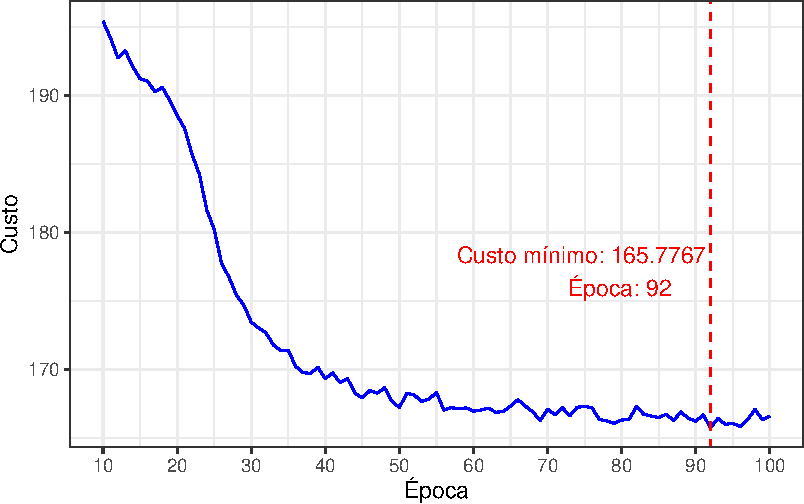
\includegraphics{lista2-resolucao_files/figure-pdf/fig-resultadosq1-1.pdf}

}

\caption{\label{fig-resultadosq1}Custo no conjunto de treinamento}

\end{figure}%

~

O vetor gradiente obtido na melhor época é

\begin{verbatim}
       w1        w2        w3        w4        w5        w6        b1        b2 
 1.313836  1.316983 -5.631248 -5.639386  8.835846  8.874542 -2.348411 -2.356765 
       b3 
18.454321 
\end{verbatim}

~

\subsection{Item b)}\label{item-b}

Considerando os pesos obtidos na Seção~\ref{sec-1a}, para a primeira
observação do conjunto de teste, gere 200 previsões
\((\hat{y}_{1,1} , \dots , \hat{y}_{1,200})\), uma para cada sub-rede
amostrada aleatoriamente. Use as previsões para construir uma estimativa
pontual e um intervalo de confiança para \(y_1\) . Veja a Figura 7.6 do
livro Deep Learning. Note que com esse procedimento, não é preciso
assumir normalidade para os erros, como fizemos na Lista 1.

\begin{center}\rule{0.5\linewidth}{0.5pt}\end{center}

~

A seguir, são geradas 200 previsões para a primeira observação do
conjunto de teste, com os pesos obtidos na Seção~\ref{sec-1a}. A
previsão pontual é a média das previsões e o intervalo de confiança é
obtido empiricamente pelos quantis das previsões.

~

\begin{Shaded}
\begin{Highlighting}[]
\NormalTok{n\_pred }\OtherTok{\textless{}{-}} \DecValTok{200}
\NormalTok{predictions }\OtherTok{\textless{}{-}} \FunctionTok{numeric}\NormalTok{(n\_pred)}

\ControlFlowTok{for}\NormalTok{(i }\ControlFlowTok{in} \DecValTok{1}\SpecialCharTok{:}\NormalTok{n\_pred) \{}
\NormalTok{  predictions[i] }\OtherTok{\textless{}{-}} \FunctionTok{feed\_forward\_drop}\NormalTok{(}\AttributeTok{theta =}\NormalTok{ best\_grad, }\AttributeTok{x =}\NormalTok{ x\_teste[}\DecValTok{1}\NormalTok{,])}
\NormalTok{\}}
\end{Highlighting}
\end{Shaded}

~

A estimativa pontual e o intervalo de confiança são dados a seguir:

~

\begin{Shaded}
\begin{Highlighting}[]
\NormalTok{mean\_pred }\OtherTok{\textless{}{-}} \FunctionTok{mean}\NormalTok{(predictions)}
\FunctionTok{quantile}\NormalTok{(predictions, }\FunctionTok{c}\NormalTok{(}\FloatTok{0.025}\NormalTok{, }\FloatTok{0.975}\NormalTok{))}
\end{Highlighting}
\end{Shaded}

\begin{verbatim}
    2.5%    97.5% 
18.45432 24.18317 
\end{verbatim}

~

As previsões geradas estão representadas na
Figura~\ref{fig-previsoesq1b}. A linha vermelha representa a média e as
linhas azuis representam os limites do intervalo de confiança.

~

\begin{Shaded}
\begin{Highlighting}[]
\NormalTok{data\_plot\_q1b }\OtherTok{\textless{}{-}} \FunctionTok{tibble}\NormalTok{(}
  \AttributeTok{pred =}\NormalTok{ predictions}
\NormalTok{)}

\FunctionTok{ggplot}\NormalTok{(data\_plot\_q1b) }\SpecialCharTok{+}
  \FunctionTok{geom\_histogram}\NormalTok{(}\FunctionTok{aes}\NormalTok{(}\AttributeTok{x =}\NormalTok{ pred), }\AttributeTok{bins =} \DecValTok{30}\NormalTok{) }\SpecialCharTok{+}
  \FunctionTok{geom\_vline}\NormalTok{(}\AttributeTok{xintercept =}\NormalTok{ mean\_pred, }\AttributeTok{linetype =} \StringTok{"dashed"}\NormalTok{, }\AttributeTok{color =} \StringTok{"red"}\NormalTok{) }\SpecialCharTok{+}
  \FunctionTok{geom\_vline}\NormalTok{(}\AttributeTok{xintercept =} \FunctionTok{quantile}\NormalTok{(predictions, }\FloatTok{0.025}\NormalTok{), }\AttributeTok{linetype =} \StringTok{"dashed"}\NormalTok{, }\AttributeTok{color =} \StringTok{"blue"}\NormalTok{) }\SpecialCharTok{+}
  \FunctionTok{geom\_vline}\NormalTok{(}\AttributeTok{xintercept =} \FunctionTok{quantile}\NormalTok{(predictions, }\FloatTok{0.975}\NormalTok{), }\AttributeTok{linetype =} \StringTok{"dashed"}\NormalTok{, }\AttributeTok{color =} \StringTok{"blue"}\NormalTok{) }\SpecialCharTok{+}
  \FunctionTok{scale\_y\_continuous}\NormalTok{(}\AttributeTok{expand =} \FunctionTok{c}\NormalTok{(}\DecValTok{0}\NormalTok{, }\DecValTok{0}\NormalTok{)) }\SpecialCharTok{+}
  \FunctionTok{labs}\NormalTok{(}
    \AttributeTok{x =} \StringTok{"Previsões"}\NormalTok{,}
    \AttributeTok{y =} \StringTok{"Frequência"}
\NormalTok{  ) }\SpecialCharTok{+}
  \FunctionTok{theme\_bw}\NormalTok{()}
\end{Highlighting}
\end{Shaded}

\begin{figure}[H]

\centering{

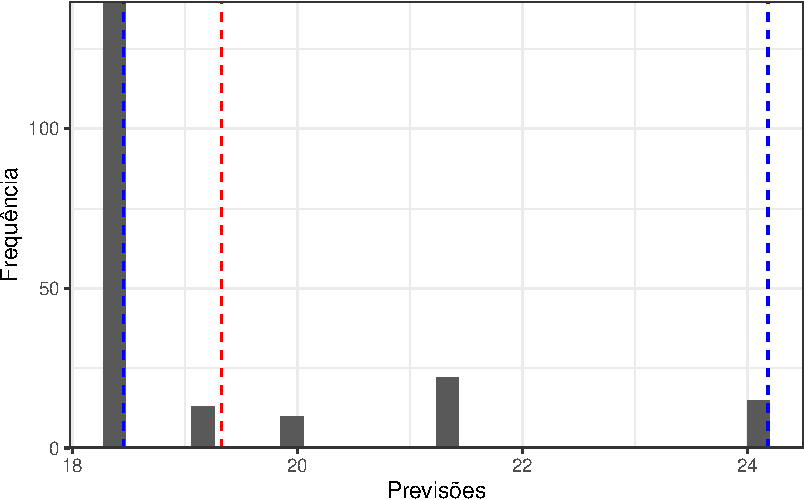
\includegraphics{lista2-resolucao_files/figure-pdf/fig-previsoesq1b-1.pdf}

}

\caption{\label{fig-previsoesq1b}Previsões para a primeira observação do
conjunto de teste}

\end{figure}%

~

\subsection{Item c)}\label{item-c}

Repita o item b) para gerar estimativas pontuais para cada observação do
conjunto de testes.

\begin{center}\rule{0.5\linewidth}{0.5pt}\end{center}

~

Usando o mesmo vetor gradiente obtido na Seção~\ref{sec-1a}, são geradas
previsões para cada observação do conjunto de teste.

~

\begin{Shaded}
\begin{Highlighting}[]
\CommentTok{\#ajuste do tamanho das predições}
\NormalTok{n\_pred }\OtherTok{\textless{}{-}} \DecValTok{200}

\CommentTok{\#monta uma lista de previsões para cada observação}
\NormalTok{pred\_matrix\_drop }\OtherTok{\textless{}{-}} \FunctionTok{replicate}\NormalTok{(}\AttributeTok{n =} \FunctionTok{nrow}\NormalTok{(x\_teste), }\AttributeTok{expr =} \FunctionTok{rep}\NormalTok{(}\DecValTok{0}\NormalTok{, n\_pred), }\AttributeTok{simplify =} \ConstantTok{FALSE}\NormalTok{)}

\ControlFlowTok{for}\NormalTok{(j }\ControlFlowTok{in} \DecValTok{1}\SpecialCharTok{:}\FunctionTok{nrow}\NormalTok{(x\_teste)) \{ }\CommentTok{\# 1:10000 elementos do conjunto de teste}
  \ControlFlowTok{for}\NormalTok{(i }\ControlFlowTok{in} \DecValTok{1}\SpecialCharTok{:}\NormalTok{n\_pred) \{ }\CommentTok{\# 1:200 predições para cada elemento do conjunto de teste}
\NormalTok{    pred\_matrix\_drop[[j]][i] }\OtherTok{\textless{}{-}} \FunctionTok{feed\_forward\_drop}\NormalTok{(}\AttributeTok{theta =}\NormalTok{ best\_grad, }\AttributeTok{x =}\NormalTok{ x\_teste[j,])}
\NormalTok{  \}}
\NormalTok{\}}

\NormalTok{means\_q1c }\OtherTok{\textless{}{-}} \FunctionTok{sapply}\NormalTok{(pred\_matrix\_drop, mean)}
\end{Highlighting}
\end{Shaded}

~

\subsection{Item d)}\label{item-d}

Use a regra weight scaling inference rule (página 263 do livro Deep
Learning) para gerar novas estimativas para as observações do conjunto
de testes. Qual dos procedimentos (o do item c) ou o utilizado neste
item) produziu melhores resultados? Considerando o tempo computacional
de cada um, qual você escolheria nessa aplicação?

\begin{center}\rule{0.5\linewidth}{0.5pt}\end{center}

~

Primeiro são obtidas as previsões usando WSIR. A diferença entre esse
método e o anterior é

\[
\begin{aligned}
  \mathbf{W}_{(.)}^{\text{WSIR}} &= p \mathbf{W}_{(.)} \\
  \mathbf{A} &= \mathbf{b}_1 + \mathbf{W}_{(.)}^{\text{WSIR}} \mathbf{X} \\
  \mathbf{\hat{y}} &= \mathbf{H} \mathbf{W}_2^{\text{WSIR}} + b_3
\end{aligned}
\] ~

Em seguida, recalibramos a rede com a mesma inicialização, mas usando
WSIR. Em seguida, geramos novamente 200 previsões para cada observação
do conjunto de teste com o melhor \(\boldsymbol{\theta}_{\text{WSIR}}\).

~

\begin{Shaded}
\begin{Highlighting}[]
\NormalTok{epsilon }\OtherTok{\textless{}{-}} \FloatTok{0.1}
\NormalTok{M }\OtherTok{\textless{}{-}} \DecValTok{100}

\CommentTok{\#lista de theta para receber os valores}
\NormalTok{theta\_est\_WSIR }\OtherTok{\textless{}{-}} \FunctionTok{list}\NormalTok{()}
\CommentTok{\# Theta inicial}
\NormalTok{theta\_est\_WSIR[[}\DecValTok{1}\NormalTok{]] }\OtherTok{\textless{}{-}} \FunctionTok{rep}\NormalTok{(}\DecValTok{0}\NormalTok{, }\DecValTok{9}\NormalTok{)}
\CommentTok{\# inicializacao do vetor de custo}
\NormalTok{custo\_treino\_WSIR }\OtherTok{\textless{}{-}} \FunctionTok{numeric}\NormalTok{(M)}


\CommentTok{\# Execução}
\ControlFlowTok{for}\NormalTok{(i }\ControlFlowTok{in} \DecValTok{1}\SpecialCharTok{:}\NormalTok{M) \{}
\CommentTok{\# Cálculo dos gradientes dos parâmetros}
\NormalTok{  grad }\OtherTok{\textless{}{-}} \FunctionTok{back\_prop\_weight}\NormalTok{(}\AttributeTok{theta =}\NormalTok{ theta\_est\_WSIR[[i]], }\AttributeTok{x =}\NormalTok{ x\_treino, }\AttributeTok{y =}\NormalTok{ y\_treino)}
  \CommentTok{\# Cálculo do custo de treino}
\NormalTok{  custo\_treino\_WSIR[i] }\OtherTok{\textless{}{-}}\NormalTok{ grad}\SpecialCharTok{$}\NormalTok{mse\_cost}
  \CommentTok{\# Atualização dos parâmetros}
\NormalTok{  theta\_est\_WSIR[[i}\SpecialCharTok{+}\DecValTok{1}\NormalTok{]] }\OtherTok{\textless{}{-}}\NormalTok{ theta\_est\_WSIR[[i]] }\SpecialCharTok{{-}}\NormalTok{ epsilon}\SpecialCharTok{*}\NormalTok{grad}\SpecialCharTok{$}\NormalTok{vetor\_grad}
\NormalTok{\}}

\NormalTok{best\_epoch\_WSIR }\OtherTok{\textless{}{-}} \FunctionTok{which}\NormalTok{(custo\_treino\_WSIR }\SpecialCharTok{==} \FunctionTok{min}\NormalTok{(custo\_treino\_WSIR))}
\NormalTok{min\_cost\_WSIR }\OtherTok{\textless{}{-}} \FunctionTok{min}\NormalTok{(custo\_treino\_WSIR)}
\NormalTok{best\_grad\_WSIR }\OtherTok{\textless{}{-}}\NormalTok{ theta\_est\_WSIR[[best\_epoch\_WSIR]]}

\CommentTok{\#ajuste do tamanho das predições}
\NormalTok{n\_pred }\OtherTok{\textless{}{-}} \DecValTok{200}

\CommentTok{\#monta uma lista de previsões para cada observação}
\NormalTok{pred\_matrix\_WSIR }\OtherTok{\textless{}{-}} \FunctionTok{replicate}\NormalTok{(}\AttributeTok{n =} \FunctionTok{nrow}\NormalTok{(x\_teste), }\AttributeTok{expr =} \FunctionTok{rep}\NormalTok{(}\DecValTok{0}\NormalTok{, n\_pred), }\AttributeTok{simplify =} \ConstantTok{FALSE}\NormalTok{)}

\ControlFlowTok{for}\NormalTok{(j }\ControlFlowTok{in} \DecValTok{1}\SpecialCharTok{:}\FunctionTok{nrow}\NormalTok{(x\_teste)) \{ }\CommentTok{\# 1:10000 elementos do conjunto de teste}
  \ControlFlowTok{for}\NormalTok{(i }\ControlFlowTok{in} \DecValTok{1}\SpecialCharTok{:}\NormalTok{n\_pred) \{ }\CommentTok{\# 1:200 predições para cada elemento do conjunto de teste}
\NormalTok{    pred\_matrix\_WSIR[[j]][i] }\OtherTok{\textless{}{-}} \FunctionTok{feed\_forward\_scale}\NormalTok{(}\AttributeTok{theta =}\NormalTok{ best\_grad\_WSIR, }\AttributeTok{x =}\NormalTok{ x\_teste[j,])}
\NormalTok{  \}}
\NormalTok{\}}

\NormalTok{means\_q1d }\OtherTok{\textless{}{-}} \FunctionTok{sapply}\NormalTok{(pred\_matrix\_WSIR, mean)}
\end{Highlighting}
\end{Shaded}

~

Com base estritamente no MSE, o método drop-out produziu melhores
resultados, como mostrado na Tabela~\ref{tbl-mseq1cd}.

~

\begin{longtable}[]{@{}lr@{}}

\caption{\label{tbl-mseq1cd}MSE no conjunto de teste}

\tabularnewline

\toprule\noalign{}
Metodo & MSE \\
\midrule\noalign{}
\endhead
\bottomrule\noalign{}
\endlastfoot
Dropout & 143.48 \\
WSIR & 214.25 \\

\end{longtable}

~

\section{Questão 2}\label{questuxe3o-2}

A questão 2 foi realizada no
\href{https://colab.research.google.com/drive/1cYhcgZacw-x59x6bCt2duFvGixKCIALB?usp=sharing}{Google
Collab}. A maior parte dos resultados desta seção foram obtidos a partir
de uma sessão na plataforma.

~

\subsection{Item a)}\label{item-a}

Ajuste a rede neural especificada na Lista 1 usando o \emph{Keras}.
Compare com sua implementação (Lista 1, item e) quanto ao tempo
computacional e ao custo obtido no conjunto de validação. Use o mesmo
algoritmo de otimização (\emph{full gradient descent}) e ponto de
partida.

\begin{center}\rule{0.5\linewidth}{0.5pt}\end{center}

Primeiro foram instalados os pacotes necessários: ~

\begin{Shaded}
\begin{Highlighting}[]
\FunctionTok{install.packages}\NormalTok{(}\StringTok{"pacman"}\NormalTok{)}
\NormalTok{pacman}\SpecialCharTok{::}\FunctionTok{p\_load}\NormalTok{(}\StringTok{"tidyverse"}\NormalTok{, }\StringTok{"keras"}\NormalTok{, }\StringTok{"tensorflow"}\NormalTok{, }\StringTok{"reticulate"}\NormalTok{, }\StringTok{"rsample"}\NormalTok{)}
\end{Highlighting}
\end{Shaded}

~

Os dados utilizados foram iguais aos utilizados na sessão local:

\begin{Shaded}
\begin{Highlighting}[]
\DocumentationTok{\#\#\# Configurações iniciais {-}{-}{-}{-}}
\CommentTok{\# semente aleatoria indicada}
\FunctionTok{set.seed}\NormalTok{(}\FloatTok{1.2024}\NormalTok{)}

\DocumentationTok{\#\#\# Gerando dados "observados"}
\NormalTok{m.obs }\OtherTok{\textless{}{-}} \DecValTok{100000}
\NormalTok{dados }\OtherTok{\textless{}{-}} \FunctionTok{tibble}\NormalTok{(}\AttributeTok{x1.obs=}\FunctionTok{runif}\NormalTok{(m.obs, }\SpecialCharTok{{-}}\DecValTok{3}\NormalTok{, }\DecValTok{3}\NormalTok{),}
                \AttributeTok{x2.obs=}\FunctionTok{runif}\NormalTok{(m.obs, }\SpecialCharTok{{-}}\DecValTok{3}\NormalTok{, }\DecValTok{3}\NormalTok{)) }\SpecialCharTok{\%\textgreater{}\%}
         \FunctionTok{mutate}\NormalTok{(}\AttributeTok{mu=}\FunctionTok{abs}\NormalTok{(x1.obs}\SpecialCharTok{\^{}}\DecValTok{3} \SpecialCharTok{{-}} \DecValTok{30}\SpecialCharTok{*}\FunctionTok{sin}\NormalTok{(x2.obs) }\SpecialCharTok{+} \DecValTok{10}\NormalTok{),}
                \AttributeTok{y=}\FunctionTok{rnorm}\NormalTok{(m.obs, }\AttributeTok{mean=}\NormalTok{mu, }\AttributeTok{sd=}\DecValTok{1}\NormalTok{))}

\CommentTok{\# dados particionados conforme a lista 1}
\NormalTok{treino }\OtherTok{\textless{}{-}}\NormalTok{ dados[}\DecValTok{1}\SpecialCharTok{:}\DecValTok{80000}\NormalTok{, ]}
\NormalTok{val }\OtherTok{\textless{}{-}}\NormalTok{ dados[}\DecValTok{80001}\SpecialCharTok{:}\DecValTok{90000}\NormalTok{, ]}
\NormalTok{teste }\OtherTok{\textless{}{-}}\NormalTok{ dados[}\DecValTok{90001}\SpecialCharTok{:}\FunctionTok{nrow}\NormalTok{(dados), ]}

\CommentTok{\# particoes de x}
\NormalTok{x\_treino }\OtherTok{\textless{}{-}}\NormalTok{ treino }\SpecialCharTok{\%\textgreater{}\%}
  \FunctionTok{select}\NormalTok{(x1.obs, x2.obs) }\SpecialCharTok{\%\textgreater{}\%}
  \FunctionTok{as.matrix}\NormalTok{()}
\NormalTok{x\_val }\OtherTok{\textless{}{-}}\NormalTok{ val }\SpecialCharTok{\%\textgreater{}\%}
  \FunctionTok{select}\NormalTok{(x1.obs, x2.obs) }\SpecialCharTok{\%\textgreater{}\%}
  \FunctionTok{as.matrix}\NormalTok{()}
\NormalTok{x\_teste }\OtherTok{\textless{}{-}}\NormalTok{ teste }\SpecialCharTok{\%\textgreater{}\%}
  \FunctionTok{select}\NormalTok{(x1.obs, x2.obs) }\SpecialCharTok{\%\textgreater{}\%}
  \FunctionTok{as.matrix}\NormalTok{()}

\CommentTok{\# particoes de y}
\NormalTok{y\_treino }\OtherTok{\textless{}{-}}\NormalTok{ treino}\SpecialCharTok{$}\NormalTok{y}
\NormalTok{y\_val }\OtherTok{\textless{}{-}}\NormalTok{ val}\SpecialCharTok{$}\NormalTok{y}
\NormalTok{y\_teste }\OtherTok{\textless{}{-}}\NormalTok{ teste}\SpecialCharTok{$}\NormalTok{y}
\end{Highlighting}
\end{Shaded}

~

Em seguida, o modelo é configurado. O full gradient descent, de acordo
com a documentação, é obtido com as configurações
\texttt{lr\ =\ 0.1,\ momentum\ =\ 0,\ weight\_decay\ =\ FALSE)} do
otimizador. A função de ativação é definida como sigmóide e
\texttt{kernel\_initializer=\textquotesingle{}zeros\textquotesingle{},\ bias\_initializer=\textquotesingle{}zeros\textquotesingle{}}
indicam a inicialização dos pesos e dos viéses como zero. Finalmente, a
métrica da função perda é definida como MSE. ~

\begin{Shaded}
\begin{Highlighting}[]
\CommentTok{\# definicao do modelo}
\NormalTok{model }\OtherTok{\textless{}{-}} \FunctionTok{keras\_model\_sequential}\NormalTok{() }\SpecialCharTok{\%\textgreater{}\%}
  \FunctionTok{layer\_dense}\NormalTok{(}\AttributeTok{units =} \DecValTok{2}\NormalTok{, }\AttributeTok{input\_shape =} \FunctionTok{c}\NormalTok{(}\DecValTok{2}\NormalTok{), }\AttributeTok{activation =} \StringTok{\textquotesingle{}sigmoid\textquotesingle{}}\NormalTok{, }\AttributeTok{kernel\_initializer=}\StringTok{\textquotesingle{}zeros\textquotesingle{}}\NormalTok{, }\AttributeTok{bias\_initializer=}\StringTok{\textquotesingle{}zeros\textquotesingle{}}\NormalTok{) }\SpecialCharTok{\%\textgreater{}\%}
  \FunctionTok{layer\_dense}\NormalTok{(}\AttributeTok{units =} \DecValTok{1}\NormalTok{)}

\CommentTok{\# compilar o modelo com full gradient descent}
\NormalTok{model }\SpecialCharTok{\%\textgreater{}\%} \FunctionTok{compile}\NormalTok{(}
  \AttributeTok{optimizer =} \FunctionTok{optimizer\_sgd}\NormalTok{(}\AttributeTok{lr =} \FloatTok{0.1}\NormalTok{, }\AttributeTok{momentum =} \DecValTok{0}\NormalTok{, }\AttributeTok{weight\_decay =} \ConstantTok{FALSE}\NormalTok{),  }\CommentTok{\# Gradient descent with learning rate 0.01}
  \AttributeTok{loss =} \StringTok{\textquotesingle{}mse\textquotesingle{}}\NormalTok{,}
  \AttributeTok{metrics =} \StringTok{\textquotesingle{}mse\textquotesingle{}}
\NormalTok{)}
\end{Highlighting}
\end{Shaded}

~

O modelo é entao treinado com 100 épocas e o \emph{batch} é definido
como o tamanho total do banco de dados. As partições específicas de
treino e validação são definidas.

~

\begin{Shaded}
\begin{Highlighting}[]
\NormalTok{history }\OtherTok{\textless{}{-}}\NormalTok{ model }\SpecialCharTok{\%\textgreater{}\%} \FunctionTok{fit}\NormalTok{(}
  \AttributeTok{x =}\NormalTok{ x\_treino,}
  \AttributeTok{y =}\NormalTok{ y\_treino,}
  \AttributeTok{epochs =} \DecValTok{100}\NormalTok{,        }
  \AttributeTok{batch\_size =} \FunctionTok{nrow}\NormalTok{(x\_treino),  }
  \AttributeTok{validation\_data =} \FunctionTok{list}\NormalTok{(x\_val, y\_val), }
  \AttributeTok{verbose =} \DecValTok{2}
\NormalTok{)}
\end{Highlighting}
\end{Shaded}

~

Finalmente, obtém-se os pesos e o custo associado a esse modelo no
conjunto de validação.

~

\begin{Shaded}
\begin{Highlighting}[]
\NormalTok{evaluation }\OtherTok{\textless{}{-}}\NormalTok{ model }\SpecialCharTok{\%\textgreater{}\%} \FunctionTok{evaluate}\NormalTok{(x\_val, y\_val, }\AttributeTok{verbose =} \DecValTok{0}\NormalTok{)}

\NormalTok{mse\_loss }\OtherTok{\textless{}{-}}\NormalTok{ evaluation[[}\StringTok{\textquotesingle{}loss\textquotesingle{}}\NormalTok{]]}

\NormalTok{weights\_model1 }\OtherTok{\textless{}{-}}\NormalTok{ model }\SpecialCharTok{\%\textgreater{}\%} \FunctionTok{get\_weights}\NormalTok{()}
\end{Highlighting}
\end{Shaded}

O tempo de treino foi de 11 segundos e o menor custo observado foi de
142.8076477. O tempo de treino é muito próximo ao item e) da lista 1,
assim como o custo. Os pesos obtidos foram:

\begin{verbatim}
[[1]]
           [,1]       [,2]
[1,] -0.8902205 -0.9162572
[2,] -2.0196459 -2.0407729

[[2]]
[1] 2.463278 2.528810

[[3]]
         [,1]
[1,] 8.927702
[2,] 9.146015

[[4]]
[1] 8.982577
\end{verbatim}

~

\subsection{Item b)}\label{item-b-1}

Ajuste a rede neural mais precisa (medida pelo MSE calculado sobre o
conjunto de validação) que conseguir, com a arquitetura que quiser. Use
todos os artifícios de regularização que desejar (\emph{weight decay},
\emph{Bagging}, \emph{droupout}, \emph{Early stopping}). Reporte a
precisão obtida para essa rede no conjunto de validação.

\begin{center}\rule{0.5\linewidth}{0.5pt}\end{center}

~

Optou-se por uma arquitetura de rede com 3 camadas intermediárias
\emph{fully connected} com 128 unidades cada, função de ativação ReLU e
inicialização aleatória dos pesos. A regularização \emph{dropout} foi
aplicada com probabilidade de 0,5. O otimizador escolhido foi o
\emph{Adam} com taxa de aprendizado de 0,01 e \emph{minibatch} de
tamanho 32 para 100 épocas. O modelo foi treinado com 1000 épocas e
\emph{batch} de tamanho 32.

~

\begin{Shaded}
\begin{Highlighting}[]
\NormalTok{model2 }\OtherTok{\textless{}{-}} \FunctionTok{keras\_model\_sequential}\NormalTok{() }\SpecialCharTok{\%\textgreater{}\%}
  \FunctionTok{layer\_dense}\NormalTok{(}\AttributeTok{units =} \DecValTok{128}\NormalTok{, }\AttributeTok{input\_shape =} \FunctionTok{c}\NormalTok{(}\DecValTok{2}\NormalTok{), }\AttributeTok{activation =} \StringTok{\textquotesingle{}relu\textquotesingle{}}\NormalTok{) }\SpecialCharTok{\%\textgreater{}\%}
  \FunctionTok{layer\_dropout}\NormalTok{(}\AttributeTok{rate =} \FloatTok{0.5}\NormalTok{) }\SpecialCharTok{\%\textgreater{}\%}  
  \FunctionTok{layer\_dense}\NormalTok{(}\AttributeTok{units =} \DecValTok{128}\NormalTok{, }\AttributeTok{activation =} \StringTok{\textquotesingle{}relu\textquotesingle{}}\NormalTok{) }\SpecialCharTok{\%\textgreater{}\%}
  \FunctionTok{layer\_dropout}\NormalTok{(}\AttributeTok{rate =} \FloatTok{0.5}\NormalTok{) }\SpecialCharTok{\%\textgreater{}\%}  
  \FunctionTok{layer\_dense}\NormalTok{(}\AttributeTok{units =} \DecValTok{128}\NormalTok{, }\AttributeTok{activation =} \StringTok{\textquotesingle{}relu\textquotesingle{}}\NormalTok{) }\SpecialCharTok{\%\textgreater{}\%}
  \FunctionTok{layer\_dropout}\NormalTok{(}\AttributeTok{rate =} \FloatTok{0.5}\NormalTok{) }\SpecialCharTok{\%\textgreater{}\%}  
  \FunctionTok{layer\_dense}\NormalTok{(}\AttributeTok{units =} \DecValTok{1}\NormalTok{)  }

\NormalTok{model2 }\SpecialCharTok{\%\textgreater{}\%} \FunctionTok{compile}\NormalTok{(}
  \AttributeTok{optimizer =} \FunctionTok{optimizer\_adam}\NormalTok{(}\AttributeTok{lr =} \FloatTok{0.01}\NormalTok{),  }
  \AttributeTok{loss =} \StringTok{\textquotesingle{}mse\textquotesingle{}}\NormalTok{,}
  \AttributeTok{metrics =} \StringTok{\textquotesingle{}mse\textquotesingle{}}
\NormalTok{)}

\NormalTok{history2 }\OtherTok{\textless{}{-}}\NormalTok{ model2 }\SpecialCharTok{\%\textgreater{}\%} \FunctionTok{fit}\NormalTok{(}
  \AttributeTok{x =}\NormalTok{ x\_treino,}
  \AttributeTok{y =}\NormalTok{ y\_treino,}
  \AttributeTok{epochs =} \DecValTok{100}\NormalTok{,          }
  \AttributeTok{batch\_size =} \DecValTok{32}\NormalTok{,       }
  \AttributeTok{validation\_data =} \FunctionTok{list}\NormalTok{(x\_val, y\_val),  }
  \AttributeTok{verbose =} \DecValTok{2}
\NormalTok{)}
\end{Highlighting}
\end{Shaded}

~

O menor custo obtido no conjunto de validação, conforme indicado no
bloco a seguir, foi de 5.2935634. O tempo de treino dessa rede foi de 14
minutos.

~

\begin{Shaded}
\begin{Highlighting}[]
\NormalTok{evaluation2 }\OtherTok{\textless{}{-}}\NormalTok{ model2 }\SpecialCharTok{\%\textgreater{}\%} \FunctionTok{evaluate}\NormalTok{(x\_val, y\_val, }\AttributeTok{verbose =} \DecValTok{0}\NormalTok{)}

\NormalTok{mse\_loss2 }\OtherTok{\textless{}{-}}\NormalTok{ evaluation2[[}\StringTok{\textquotesingle{}loss\textquotesingle{}}\NormalTok{]]}

\NormalTok{weights\_model2 }\OtherTok{\textless{}{-}}\NormalTok{ model2 }\SpecialCharTok{\%\textgreater{}\%} \FunctionTok{get\_weights}\NormalTok{()}
\end{Highlighting}
\end{Shaded}

~

\subsection{Item c)}\label{item-c-1}

Refaça o item h) da Lista 1 para essa nova rede. Comente os resultados.

\begin{center}\rule{0.5\linewidth}{0.5pt}\end{center}

~

Este mesmo gráfico, para a lista anterior, apresentava concentrações em
valores extremos e com variância diferente em diferentes posições de
\(y\). Em comparação, a Figura~\ref{fig-previsoesq2c} apresenta uma
distribuição mais homocedástica e com valores mais próximos de \(y\),
evidenciado pela nuvem de pontos muito próximos à reta \(y = \hat{y}\).
É possível que a rede neural tenha sido capaz de capturar a relação
entre \(\mathbf{x}\) e \(y\) de forma mais precisa.

~

\begin{Shaded}
\begin{Highlighting}[]
\FunctionTok{tibble}\NormalTok{(}
  \AttributeTok{yhat =}\NormalTok{ nova\_y\_val,}
  \AttributeTok{y =}\NormalTok{ y\_val) }\SpecialCharTok{\%\textgreater{}\%}
  \FunctionTok{ggplot}\NormalTok{(}\FunctionTok{aes}\NormalTok{(}\AttributeTok{x =}\NormalTok{ y, }\AttributeTok{y =}\NormalTok{ yhat)) }\SpecialCharTok{+}
  \FunctionTok{geom\_point}\NormalTok{(}\AttributeTok{alpha =} \FloatTok{0.3}\NormalTok{)}\SpecialCharTok{+}
  \FunctionTok{geom\_abline}\NormalTok{(}\AttributeTok{intercept =} \DecValTok{0}\NormalTok{, }\AttributeTok{slope =} \DecValTok{1}\NormalTok{, }\AttributeTok{color =} \StringTok{"red"}\NormalTok{)}\SpecialCharTok{+}
  \FunctionTok{xlab}\NormalTok{(}\FunctionTok{TeX}\NormalTok{(}\StringTok{"$y$"}\NormalTok{)) }\SpecialCharTok{+} \FunctionTok{ylab}\NormalTok{(}\FunctionTok{TeX}\NormalTok{(}\StringTok{"$}\SpecialCharTok{\textbackslash{}\textbackslash{}}\StringTok{hat\{y\}$"}\NormalTok{))}\SpecialCharTok{+}
  \FunctionTok{theme\_bw}\NormalTok{()}
  \FunctionTok{theme}\NormalTok{(}\AttributeTok{axis.title.y =} \FunctionTok{element\_text}\NormalTok{(}\AttributeTok{angle =} \DecValTok{0}\NormalTok{, }\AttributeTok{vjust =} \FloatTok{0.5}\NormalTok{))}
\end{Highlighting}
\end{Shaded}

\begin{verbatim}
List of 1
 $ axis.title.y:List of 11
  ..$ family       : NULL
  ..$ face         : NULL
  ..$ colour       : NULL
  ..$ size         : NULL
  ..$ hjust        : NULL
  ..$ vjust        : num 0.5
  ..$ angle        : num 0
  ..$ lineheight   : NULL
  ..$ margin       : NULL
  ..$ debug        : NULL
  ..$ inherit.blank: logi FALSE
  ..- attr(*, "class")= chr [1:2] "element_text" "element"
 - attr(*, "class")= chr [1:2] "theme" "gg"
 - attr(*, "complete")= logi FALSE
 - attr(*, "validate")= logi TRUE
\end{verbatim}

\begin{figure}[H]

\centering{

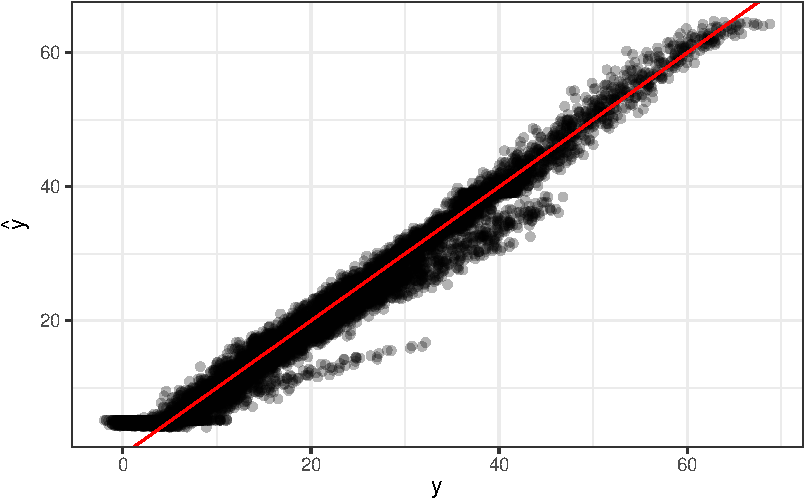
\includegraphics{lista2-resolucao_files/figure-pdf/fig-previsoesq2c-1.pdf}

}

\caption{\label{fig-previsoesq2c}Previsões para o conjunto de validação
com a rede neural do item 2b.}

\end{figure}%

~

\subsection{Item d)}\label{item-d-1}

Use a função de previsão do Keras para prever o valor da variável
resposta \(\hat{y} = f(x_1 = 1, x_2 = 1; \theta)\), para \(\theta)\)
definido de acordo com a rede ajustada. (Veja o item a) da Lista 1).

\begin{center}\rule{0.5\linewidth}{0.5pt}\end{center}

~

O valor obtido é de 14.141758. Em comparação, na lista 1 item a foi
obtido \(\hat{y}\) = 0,215.

~

\begin{Shaded}
\begin{Highlighting}[]
\NormalTok{newdata }\OtherTok{\textless{}{-}} \FunctionTok{data.frame}\NormalTok{(}\AttributeTok{x1 =} \DecValTok{1}\NormalTok{, }\AttributeTok{x2 =} \DecValTok{1}\NormalTok{) }\SpecialCharTok{\%\textgreater{}\%} \FunctionTok{as.matrix}\NormalTok{()}

\NormalTok{yhat\_d }\OtherTok{\textless{}{-}}\NormalTok{ model2 }\SpecialCharTok{\%\textgreater{}\%} \FunctionTok{predict}\NormalTok{(newdata)}

\NormalTok{yhat\_d}
\end{Highlighting}
\end{Shaded}

~

\subsection{Item e)}\label{item-e}

Neste exemplo meramente didático, conhecemos a superfície que estamos
estimando. Apresente, lado a lado, a Figura 1 da Lista 1 e a superfície
estimada pela sua rede neural. Para tanto, basta trocar a variável mu
pelos valores preditos pela rede. Comente os resultados.

\begin{center}\rule{0.5\linewidth}{0.5pt}\end{center}

~

Na Figura~\ref{fig-q2e} é exibido o gráfico da lista 1 e a superfície
estimada pela rede neural. Evidentemente a superfície de resposta não é
muito interpretável, exceto por uma possível homogeneidade de respostas.
A representação interna da rede, no entanto, parece capturar a bem a
relação entre \(x_1\), \(x_2\) e \(y\), de modo que pode ser apenas um
padrão não interpretável para o leitor.

~

\begin{Shaded}
\begin{Highlighting}[]
\CommentTok{\# figura da lista 1}
\NormalTok{n }\OtherTok{\textless{}{-}} \DecValTok{100}
\NormalTok{x1 }\OtherTok{\textless{}{-}} \FunctionTok{seq}\NormalTok{(}\SpecialCharTok{{-}}\DecValTok{3}\NormalTok{, }\DecValTok{3}\NormalTok{, }\AttributeTok{length.out=}\NormalTok{n)}
\NormalTok{x2 }\OtherTok{\textless{}{-}} \FunctionTok{seq}\NormalTok{(}\SpecialCharTok{{-}}\DecValTok{3}\NormalTok{, }\DecValTok{3}\NormalTok{, }\AttributeTok{length.out=}\NormalTok{n)}

\NormalTok{dados.superficie }\OtherTok{\textless{}{-}} \FunctionTok{as\_tibble}\NormalTok{(}\FunctionTok{expand.grid}\NormalTok{(x1, x2)) }\SpecialCharTok{\%\textgreater{}\%}
  \FunctionTok{rename\_all}\NormalTok{(}\SpecialCharTok{\textasciitilde{}} \FunctionTok{c}\NormalTok{(}\StringTok{"x1"}\NormalTok{, }\StringTok{"x2"}\NormalTok{)) }\SpecialCharTok{\%\textgreater{}\%}
  \FunctionTok{mutate}\NormalTok{(}\AttributeTok{mu =}\NormalTok{ nova\_y\_val)}

\NormalTok{plot\_superficie}\OtherTok{\textless{}{-}} \FunctionTok{ggplot}\NormalTok{(dados.superficie, }\FunctionTok{aes}\NormalTok{(}\AttributeTok{x=}\NormalTok{x1, }\AttributeTok{y=}\NormalTok{x2)) }\SpecialCharTok{+}
  \FunctionTok{geom\_point}\NormalTok{(}\FunctionTok{aes}\NormalTok{(}\AttributeTok{colour=}\NormalTok{mu), }\AttributeTok{size=}\DecValTok{2}\NormalTok{, }\AttributeTok{shape=}\DecValTok{15}\NormalTok{) }\SpecialCharTok{+}
  \FunctionTok{coord\_cartesian}\NormalTok{(}\AttributeTok{expand=}\NormalTok{F) }\SpecialCharTok{+}
  \FunctionTok{scale\_colour\_gradient2}\NormalTok{(}\AttributeTok{low=}\StringTok{"red"}\NormalTok{, }\AttributeTok{mid=}\StringTok{"white"}\NormalTok{, }\AttributeTok{high=}\StringTok{"blue"}\NormalTok{,}\CommentTok{\# midpoint=0, }
                         \AttributeTok{name=}\FunctionTok{TeX}\NormalTok{(}\StringTok{"$}\SpecialCharTok{\textbackslash{}\textbackslash{}}\StringTok{hat\{Y\}|X\_1, X\_2$"}\NormalTok{)) }\SpecialCharTok{+}
  \FunctionTok{xlab}\NormalTok{(}\FunctionTok{TeX}\NormalTok{(}\StringTok{"$X\_1$"}\NormalTok{)) }\SpecialCharTok{+} \FunctionTok{ylab}\NormalTok{(}\FunctionTok{TeX}\NormalTok{(}\StringTok{"$X\_2$"}\NormalTok{)) }\SpecialCharTok{+}
  \FunctionTok{theme}\NormalTok{(}\AttributeTok{legend.position =} \StringTok{"bottom"}\NormalTok{,}
        \AttributeTok{axis.title.y =} \FunctionTok{element\_text}\NormalTok{(}\AttributeTok{angle =} \DecValTok{0}\NormalTok{, }\AttributeTok{vjust =} \FloatTok{0.5}\NormalTok{))}

\NormalTok{dados.grid }\OtherTok{\textless{}{-}} \FunctionTok{as\_tibble}\NormalTok{(}\FunctionTok{expand.grid}\NormalTok{(x1, x2)) }\SpecialCharTok{\%\textgreater{}\%}
  \FunctionTok{rename\_all}\NormalTok{(}\SpecialCharTok{\textasciitilde{}} \FunctionTok{c}\NormalTok{(}\StringTok{"x1"}\NormalTok{, }\StringTok{"x2"}\NormalTok{)) }\SpecialCharTok{\%\textgreater{}\%}
  \FunctionTok{mutate}\NormalTok{(}\AttributeTok{mu=}\FunctionTok{abs}\NormalTok{(x1}\SpecialCharTok{\^{}}\DecValTok{3} \SpecialCharTok{{-}} \DecValTok{30}\SpecialCharTok{*}\FunctionTok{sin}\NormalTok{(x2) }\SpecialCharTok{+} \DecValTok{10}\NormalTok{))}

\NormalTok{plot\_esperanca }\OtherTok{\textless{}{-}} \FunctionTok{ggplot}\NormalTok{(dados.grid, }\FunctionTok{aes}\NormalTok{(}\AttributeTok{x=}\NormalTok{x1, }\AttributeTok{y=}\NormalTok{x2)) }\SpecialCharTok{+}
  \FunctionTok{geom\_point}\NormalTok{(}\FunctionTok{aes}\NormalTok{(}\AttributeTok{colour=}\NormalTok{mu), }\AttributeTok{size=}\DecValTok{2}\NormalTok{, }\AttributeTok{shape=}\DecValTok{15}\NormalTok{) }\SpecialCharTok{+}
  \FunctionTok{coord\_cartesian}\NormalTok{(}\AttributeTok{expand=}\NormalTok{F) }\SpecialCharTok{+}
  \FunctionTok{scale\_colour\_gradient}\NormalTok{(}\AttributeTok{low=}\StringTok{"white"}\NormalTok{,}
  \AttributeTok{high=}\StringTok{"black"}\NormalTok{,}
  \AttributeTok{name=}\FunctionTok{TeX}\NormalTok{(}\StringTok{"$E(Y|X\_1, X\_2)$"}\NormalTok{)) }\SpecialCharTok{+}
  \FunctionTok{xlab}\NormalTok{(}\FunctionTok{TeX}\NormalTok{(}\StringTok{"$X\_1$"}\NormalTok{)) }\SpecialCharTok{+} \FunctionTok{ylab}\NormalTok{(}\FunctionTok{TeX}\NormalTok{(}\StringTok{"$X\_2$"}\NormalTok{))}\SpecialCharTok{+}
  \FunctionTok{theme}\NormalTok{(}\AttributeTok{legend.position =} \StringTok{"bottom"}\NormalTok{,}
        \AttributeTok{axis.title.y =} \FunctionTok{element\_text}\NormalTok{(}\AttributeTok{angle =} \DecValTok{0}\NormalTok{, }\AttributeTok{vjust =} \FloatTok{0.5}\NormalTok{))}

\FunctionTok{plot\_grid}\NormalTok{(plot\_superficie, plot\_esperanca, }\AttributeTok{ncol=}\DecValTok{2}\NormalTok{)}
\end{Highlighting}
\end{Shaded}

\begin{figure}[H]

\centering{

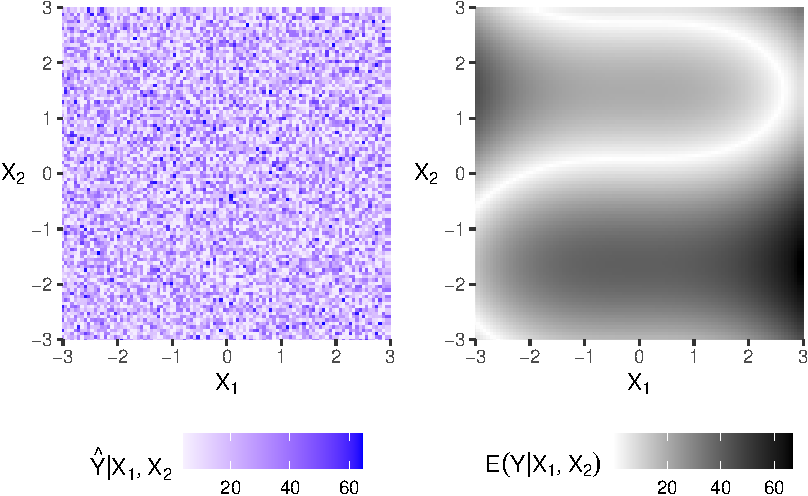
\includegraphics{lista2-resolucao_files/figure-pdf/fig-q2e-1.pdf}

}

\caption{\label{fig-q2e}Comparação entre a superfície estimada pela rede
neural e a superfície real.}

\end{figure}%

~

Para facilitar a interpretação da figura anterior, apresenta-se a
Figura~\ref{fig-q2eb} em que é exibida a superfície dos resíduos. É
notável que a maior partedos resíduos parece estar muito próxima de
zero, o que corrobora a hipótese de que a rede neural foi capaz de
capturar a relação desejada.

~

\begin{Shaded}
\begin{Highlighting}[]
\NormalTok{dados.residuos }\OtherTok{\textless{}{-}} \FunctionTok{as\_tibble}\NormalTok{(}\FunctionTok{expand.grid}\NormalTok{(x1, x2)) }\SpecialCharTok{\%\textgreater{}\%}
  \FunctionTok{rename\_all}\NormalTok{(}\SpecialCharTok{\textasciitilde{}} \FunctionTok{c}\NormalTok{(}\StringTok{"x1"}\NormalTok{, }\StringTok{"x2"}\NormalTok{)) }\SpecialCharTok{\%\textgreater{}\%}
  \FunctionTok{mutate}\NormalTok{(}\AttributeTok{mu =}\NormalTok{ nova\_y\_val}\SpecialCharTok{{-}}\NormalTok{y\_val)}

\FunctionTok{ggplot}\NormalTok{(dados.residuos, }\FunctionTok{aes}\NormalTok{(}\AttributeTok{x=}\NormalTok{x1, }\AttributeTok{y=}\NormalTok{x2)) }\SpecialCharTok{+}
  \FunctionTok{geom\_point}\NormalTok{(}\FunctionTok{aes}\NormalTok{(}\AttributeTok{colour=}\NormalTok{mu), }\AttributeTok{size=}\DecValTok{2}\NormalTok{, }\AttributeTok{shape=}\DecValTok{15}\NormalTok{) }\SpecialCharTok{+}
  \FunctionTok{coord\_cartesian}\NormalTok{(}\AttributeTok{expand=}\NormalTok{F) }\SpecialCharTok{+}
  \FunctionTok{scale\_colour\_gradient2}\NormalTok{(}\AttributeTok{low=}\StringTok{"red"}\NormalTok{, }\AttributeTok{mid=}\StringTok{"white"}\NormalTok{, }\AttributeTok{high=}\StringTok{"blue"}\NormalTok{, }\AttributeTok{midpoint=}\DecValTok{0}\NormalTok{, }
                         \AttributeTok{name=}\FunctionTok{TeX}\NormalTok{(}\StringTok{"$}\SpecialCharTok{\textbackslash{}\textbackslash{}}\StringTok{hat\{e\}|X\_1, X\_2$"}\NormalTok{)) }\SpecialCharTok{+}
  \FunctionTok{xlab}\NormalTok{(}\FunctionTok{TeX}\NormalTok{(}\StringTok{"$X\_1$"}\NormalTok{)) }\SpecialCharTok{+} \FunctionTok{ylab}\NormalTok{(}\FunctionTok{TeX}\NormalTok{(}\StringTok{"$X\_2$"}\NormalTok{)) }\SpecialCharTok{+}
  \FunctionTok{theme}\NormalTok{(}\AttributeTok{legend.position =} \StringTok{"bottom"}\NormalTok{,}
        \AttributeTok{axis.title.y =} \FunctionTok{element\_text}\NormalTok{(}\AttributeTok{angle =} \DecValTok{0}\NormalTok{, }\AttributeTok{vjust =} \FloatTok{0.5}\NormalTok{))}
\end{Highlighting}
\end{Shaded}

\begin{figure}[H]

\centering{

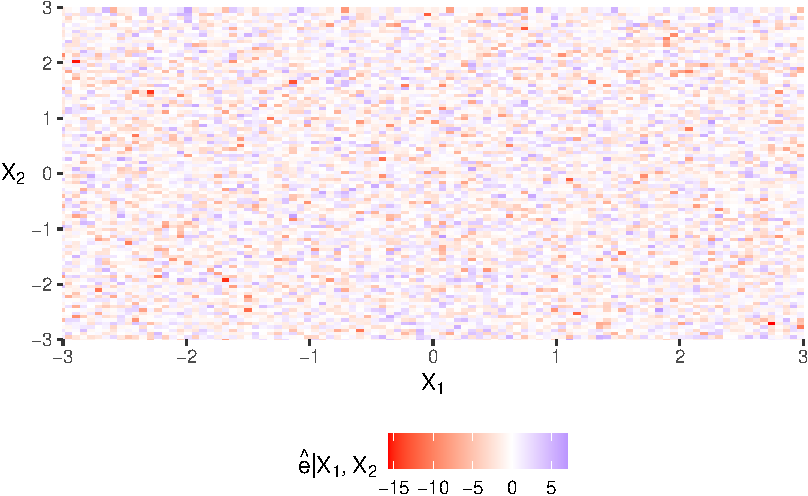
\includegraphics{lista2-resolucao_files/figure-pdf/fig-q2eb-1.pdf}

}

\caption{\label{fig-q2eb}Superfície de resíduos estimada pela rede
neural.}

\end{figure}%

~

\subsection{Item f)}\label{item-f}

Construa uma nova rede, agora ajustada sobre os valores previstos (ao
invés dos valores observados de \(y\)) para cada observação dos
conjuntos de treinamento e validação. Use a arquitetura mais
parcimoniosa que conseguir, sem comprometer substancialmente o poder de
previsão da rede (quando comparada à obtida no item 2b). Cite um
possível uso para essa nova rede.

\begin{center}\rule{0.5\linewidth}{0.5pt}\end{center}

~

Primeiro são gerados os valores previstos para cada observação dos
conjuntos de treinamento e validação.

~

\begin{Shaded}
\begin{Highlighting}[]
\NormalTok{novo\_y\_treino }\OtherTok{\textless{}{-}}\NormalTok{ model2 }\SpecialCharTok{\%\textgreater{}\%} \FunctionTok{predict}\NormalTok{(x\_treino)}
\NormalTok{nova\_y\_val }\OtherTok{\textless{}{-}}\NormalTok{ model2 }\SpecialCharTok{\%\textgreater{}\%} \FunctionTok{predict}\NormalTok{(x\_val)}
\end{Highlighting}
\end{Shaded}

~

Em seguida um novo modelo é treinado, parcimonioso em relação ao
anterior. A mudança ocorre somente na quantidade de unidades nas camadas
intermediárias, que agora é de 30 em cada uma das 3 camadas.

~

\begin{Shaded}
\begin{Highlighting}[]
\NormalTok{model3 }\OtherTok{\textless{}{-}} \FunctionTok{keras\_model\_sequential}\NormalTok{() }\SpecialCharTok{\%\textgreater{}\%}
  \FunctionTok{layer\_dense}\NormalTok{(}\AttributeTok{units =} \DecValTok{30}\NormalTok{, }\AttributeTok{input\_shape =} \FunctionTok{c}\NormalTok{(}\DecValTok{2}\NormalTok{), }\AttributeTok{activation =} \StringTok{\textquotesingle{}relu\textquotesingle{}}\NormalTok{) }\SpecialCharTok{\%\textgreater{}\%}
  \FunctionTok{layer\_dropout}\NormalTok{(}\AttributeTok{rate =} \FloatTok{0.5}\NormalTok{) }\SpecialCharTok{\%\textgreater{}\%}  
  \FunctionTok{layer\_dense}\NormalTok{(}\AttributeTok{units =} \DecValTok{30}\NormalTok{, }\AttributeTok{activation =} \StringTok{\textquotesingle{}relu\textquotesingle{}}\NormalTok{) }\SpecialCharTok{\%\textgreater{}\%}
  \FunctionTok{layer\_dropout}\NormalTok{(}\AttributeTok{rate =} \FloatTok{0.5}\NormalTok{) }\SpecialCharTok{\%\textgreater{}\%}  
  \FunctionTok{layer\_dense}\NormalTok{(}\AttributeTok{units =} \DecValTok{30}\NormalTok{, }\AttributeTok{activation =} \StringTok{\textquotesingle{}relu\textquotesingle{}}\NormalTok{) }\SpecialCharTok{\%\textgreater{}\%}
  \FunctionTok{layer\_dropout}\NormalTok{(}\AttributeTok{rate =} \FloatTok{0.5}\NormalTok{) }\SpecialCharTok{\%\textgreater{}\%}  
  \FunctionTok{layer\_dense}\NormalTok{(}\AttributeTok{units =} \DecValTok{1}\NormalTok{)  }

\NormalTok{model3 }\SpecialCharTok{\%\textgreater{}\%} \FunctionTok{compile}\NormalTok{(}
  \AttributeTok{optimizer =} \FunctionTok{optimizer\_adam}\NormalTok{(}\AttributeTok{lr =} \FloatTok{0.01}\NormalTok{),}
  \AttributeTok{loss =} \StringTok{\textquotesingle{}mse\textquotesingle{}}\NormalTok{,}
  \AttributeTok{metrics =} \StringTok{\textquotesingle{}mse\textquotesingle{}}
\NormalTok{)}

\NormalTok{history3 }\OtherTok{\textless{}{-}}\NormalTok{ model3 }\SpecialCharTok{\%\textgreater{}\%} \FunctionTok{fit}\NormalTok{(}
  \AttributeTok{x =}\NormalTok{ x\_treino,}
  \AttributeTok{y =}\NormalTok{ novo\_y\_treino,}
  \AttributeTok{epochs =} \DecValTok{100}\NormalTok{,          }
  \AttributeTok{batch\_size =} \DecValTok{32}\NormalTok{,       }
  \AttributeTok{validation\_data =} \FunctionTok{list}\NormalTok{(x\_val, nova\_y\_val),  }
  \AttributeTok{verbose =} \DecValTok{2}
\NormalTok{)}

\NormalTok{evaluation3 }\OtherTok{\textless{}{-}}\NormalTok{ model3 }\SpecialCharTok{\%\textgreater{}\%} \FunctionTok{evaluate}\NormalTok{(x\_val, nova\_y\_val, }\AttributeTok{verbose =} \DecValTok{0}\NormalTok{)}
\NormalTok{mse\_loss3 }\OtherTok{\textless{}{-}}\NormalTok{ evaluation3[[}\StringTok{\textquotesingle{}loss\textquotesingle{}}\NormalTok{]]}
\end{Highlighting}
\end{Shaded}

~

O tempo de treino foi de 12 minutos e o menor custo observado foi de
31.8574009. É possível que o as duas etapas de treinamento façam a
função de suavização de ruídos.



\end{document}
